\documentclass[12pt, twoside]{article}
\usepackage[letterpaper, margin=1in, headsep=0.5in]{geometry}
\usepackage[english]{babel}
\usepackage[utf8]{inputenc}
\usepackage{amsmath}
\usepackage{amsfonts}
\usepackage{amssymb}
\usepackage{tikz}
%\usetikzlibrary{quotes, angles}

\usepackage{graphicx}
\usepackage{enumitem}
\usepackage{multicol}

\usepackage{fancyhdr}
\pagestyle{fancy}
\fancyhf{}
\renewcommand{\headrulewidth}{0pt} % disable the underline of the header

\fancyhead[RE]{\thepage}
\fancyhead[RO]{\thepage \\ Name: \hspace{3cm}}
\fancyhead[L]{BECA / Dr. Huson / 10th Grade Geometry\\* Unit 9: Angle Relationships\\29 March 2019}

\begin{document}
\subsubsection*{9-4 Do Now Quiz: Isosceles Triangle}
  \begin{enumerate}

      \item Given isosceles $\triangle ABC$ with $\overline{AC} \cong \overline{BC}$, and $m\angle BCD=142^\circ$. Find $m\angle A$.\\[1cm]
        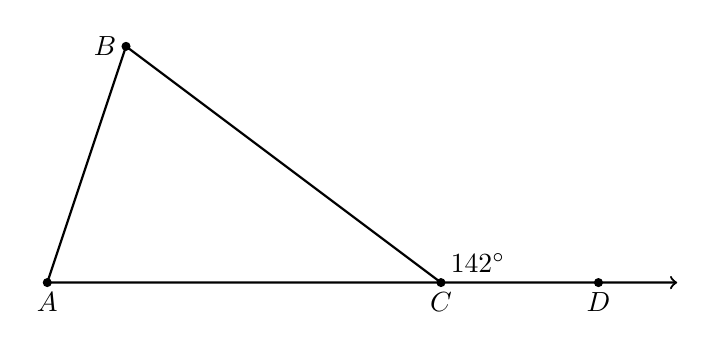
\begin{tikzpicture}
          %\draw [->, thick] (0,0)--(5,5);
          \draw [<-, thick] (8,0)--(0,0)--(1,3)--(5,0);
          \draw [fill] (0,0) circle [radius=0.05] node[below]{$A$};
          \draw [fill] (5,0) circle [radius=0.05] node[below]{$C$};
          \node at (5,0) [above right]{$142^\circ$};
          \draw [fill] (1,3) circle [radius=0.05] node[left]{$B$};
          \draw [fill] (7,0) circle [radius=0.05] node[below]{$D$};
        \end{tikzpicture}
        \vspace{3cm}

      \item In  $\triangle ABC$ shown below, side $\overline{AC}$ is extended to point $D$ with $m\angle DAB=(4x-20)^\circ$, $m\angle C=37^\circ$, and $m\angle B=(3x-20)^\circ$.
        \begin{center}
          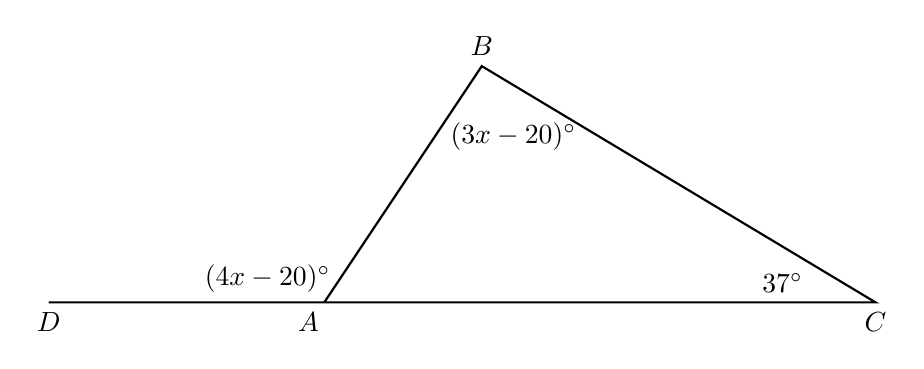
\begin{tikzpicture}
            \draw [thick](-1.5,0)node[below]{$D$}--
              (1.8,0)node[below]{$A$}--
              (9,0)node[below]{$C$}--
              (4,3)node[above]{$B$} --(2,0);
              \node at (2.2,0)[above left]{$(4x-20)^\circ$};
              \node at (8.2,0)[above left]{$37^\circ$};
              \node at (4.4,2.4)[below]{$(3x-20)^\circ$};
          \end{tikzpicture}
        \end{center}
        What is $m\angle BAC$?

\newpage
  \item Given $M(3,4)$ and $N(6,-2)$, find the length of $\overline{MN}$. Leave  the result as a simplified radical.
      \vspace{4cm}

  \item After a dilation with center $(0,0)$, the image of $\overline{ST}$ is $\overline{S'T'}$. If $ST=8.2$ and $S'T'=28.7$, find the scale factor of this dilation. \vspace{3cm}

  \item In right triangle $ABC$ shown below, point $D$ is on $\overline{AB}$ and point $E$ is on $\overline{BC}$ such that $\overline{AC} \parallel \overline{DE}$. Given $AB=21$, $BC=14$, and $EC=9$.
    \begin{center}
      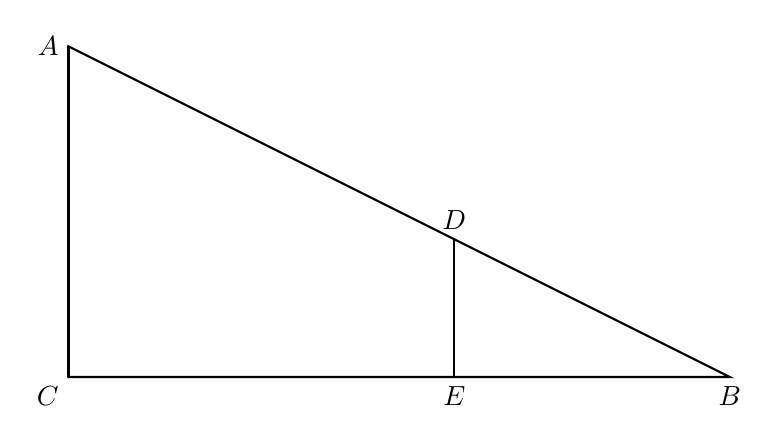
\begin{tikzpicture}[scale=0.7]
        \coordinate [label=left:$A$](A) at (-12,6);
        \coordinate [label=below:$B$](B) at (0, 0);
        \coordinate [label=below left:$C$](C) at (-12,0);
        \coordinate [label=above:$D$](D) at (-5, 2.5);
        \coordinate [label=below:$E$](E) at (-5,0);
        \draw [thick] (A)--(B)--(C)--cycle;
        \draw [thick] (A)--(C);
        \draw [thick] (D)--(E);
      \end{tikzpicture}
    \end{center}
   \begin{enumerate}
     \item Find the length of $\overline{BE}$. \vspace{0.5cm}
     \item Find the scale factor, $k$, dilating $\triangle DBE \rightarrow \triangle ABC$, centered at $B$. \vspace{1.5cm}
     \item Find $BD$.
    \end{enumerate}

\end{enumerate}


  \end{document}
